\documentclass{beamer}
\usepackage{amsmath,amssymb,amsfonts}
\usepackage{tikz}
\usetikzlibrary{calc}
\usepackage{booktabs}
\usepackage{blkarray} % For tables if needed, though likely not for a 20-min talk

% Thesis specific commands (simplified or as needed)
\newcommand{\N}{\ensuremath{\mathbb{N}}}
\newcommand{\ex}[2]{\ensuremath{\text{ex} \left( #1, #2 \right)}}
\newcommand{\compoverset}[2]{\ensuremath{K\left(#2, \overset{#1}{\dots}, #2\right)}} % k-partite, k parts of size #2
\newcommand{\compdots}[2]{\ensuremath{K\left(#1, \dots, #2\right)}} % k-partite, part sizes #1 to #2
\newcommand{\bigO}[1]{\ensuremath{\mathcal{O}\left(#1\right)}}
\newcommand{\OmegaBig}[1]{\ensuremath{\Omega\left(#1\right)}} % For asymptotic lower bound
\newcommand{\completesuperindex}[2]{\ensuremath{K^{(#1)}_{#2}}} % Complete k-graph on #2 vertices
\newcommand{\link}[3]{\ensuremath{L_{#1}\left(#2; #3\right)}} % Link graph

\title[Finding Partite Hypergraphs]{Finding Partite Hypergraphs Efficiently}
\author{Ferran Espuña Bertomeu}
\institute{Supervisor: Richard Lang}
\date{June 2025 (Presentation Adaptation)}

\usetheme{Madrid} % A common Beamer theme; choose any you like
\usecolortheme{default}

\begin{document}

% --- Title Slide ---
\begin{frame}
  \titlepage
\end{frame}

% --- Outline Slide ---
\begin{frame}{Outline}
  \tableofcontents
\end{frame}

% --- Section 1: Introduction ---
\section{Introduction}

\begin{frame}{What are Hypergraphs?}
  \begin{itemize}
    \item A \textbf{hypergraph} $G=(V,E)$ consists of a set of vertices $V$ and a set of edges $E$, where each edge is a subset of $V$.
    \pause
    \item A \textbf{$k$-uniform hypergraph} (or $k$-graph) is one where all edges have size $k$.
    \begin{itemize}
        \item $1$-graph: a subset of $V$.
        \item $2$-graph: a simple graph.
    \end{itemize}
    \pause
    \item \textbf{Applications}: Combinatorics, computer science, data analysis, biology.
  \end{itemize}
  \vfill
  \begin{columns}[T]
    \begin{column}{0.45\textwidth}
      \centering
      A 2-graph (graph):\\
      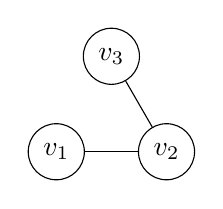
\begin{tikzpicture}[scale=0.7]
        \node[draw,circle] (v1) at (0,0) {$v_1$};
        \node[draw,circle] (v2) at (2,0) {$v_2$};
        \node[draw,circle] (v3) at (1,1.732) {$v_3$};
        \draw (v1) -- (v2);
        \draw (v2) -- (v3);
      \end{tikzpicture}
    \end{column}
    \begin{column}{0.45\textwidth}
      \centering
      A 3-graph:\\
      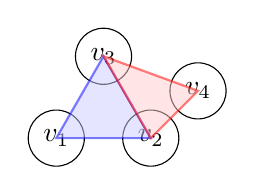
\begin{tikzpicture}[scale=0.6]
        \node[draw,circle] (v1) at (0,0) {$v_1$};
        \node[draw,circle] (v2) at (2,0) {$v_2$};
        \node[draw,circle] (v3) at (1,1.732) {$v_3$};
        \node[draw,circle] (v4) at (3,1) {$v_4$};
        \draw[thick, blue, fill=blue!20, opacity=0.5] (v1.center) -- (v2.center) -- (v3.center) -- cycle; % Edge {v1,v2,v3}
        \draw[thick, red, fill=red!20, opacity=0.5] (v2.center) -- (v3.center) -- (v4.center) -- cycle;   % Edge {v2,v3,v4}
      \end{tikzpicture}
    \end{column}
  \end{columns}
\end{frame}

\begin{frame}{Extremal Problems & Turán Numbers}
  \begin{itemize}
    \item \textbf{Extremal (Hyper)Graph Theory}: Studies maximum/minimum size of structures with certain properties.
    \pause
    \item \textbf{Turán-type problem}: Given a $k$-graph $F$ (forbidden subgraph), what is the maximum number of edges, $\ex{n}{F}$, a $k$-graph on $n$ vertices can have without containing $F$?
    \pause
    \item \textbf{Turán's Theorem (Graphs, $k=2$)}: Determines $\ex{n}{\completesuperindex{2}{r}}$.
    \pause
    \item \textbf{Turán density}: $\pi(F) = \lim_{n \to \infty} \frac{\ex{n}{F}}{\binom{n}{k}}$.
    \begin{itemize}
        \item $\pi(F) > 0$: "Non-degenerate" problem.
        \item $\pi(F) = 0$: "Degenerate" problem. This occurs if and only if $F$ is $k$-partite.
    \end{itemize}
    \pause
    \item \textbf{This thesis focuses on the degenerate case $\pi(F)=0$.}
  \end{itemize}
\end{frame}

\begin{frame}{Focus: Complete $k$-partite $k$-graphs}
  \begin{itemize}
    \item A $k$-graph $F$ is \textbf{$k$-partite} if $V(F)$ can be partitioned into $V_1, \dots, V_k$ such that every edge contains at most one vertex from each $V_i$ (actually, exactly one if $F$ has edges).
    \pause
    \item We focus on \textbf{complete balanced $k$-partite $k$-graphs}, denoted $\compoverset{k}{t}$.
    \begin{itemize}
        \item $k$ disjoint sets of $t$ vertices each ($V_1, \dots, V_k$, with $|V_i|=t$).
        \item All $t^k$ possible edges (one vertex from each part).
    \end{itemize}
  \end{itemize}
  \pause
  \centering
  Example: $\compoverset{3}{2}$ (or $K(2,2,2)$)
  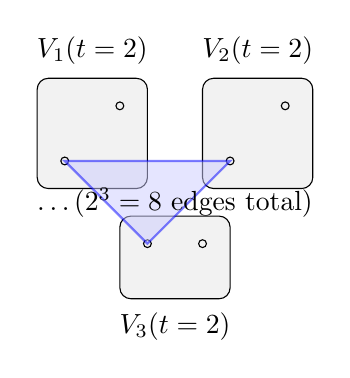
\begin{tikzpicture}[scale=0.7]
     \draw[fill=gray!10, rounded corners] (-0.5,-0.5) rectangle (1.5,1.5); \node at (0.5,2) {$V_1 (t=2)$};
     \draw[fill=gray!10, rounded corners] (2.5,-0.5) rectangle (4.5,1.5); \node at (3.5,2) {$V_2 (t=2)$};
     \draw[fill=gray!10, rounded corners] (1,-2.5) rectangle (3,-1); \node at (2,-3) {$V_3 (t=2)$};
     \node[draw,circle,inner sep=1pt] (v1a) at (0,0) {}; \node[draw,circle,inner sep=1pt] (v1b) at (1,1) {};
     \node[draw,circle,inner sep=1pt] (v2a) at (3,0) {}; \node[draw,circle,inner sep=1pt] (v2b) at (4,1) {};
     \node[draw,circle,inner sep=1pt] (v3a) at (1.5,-1.5) {}; \node[draw,circle,inner sep=1pt] (v3b) at (2.5,-1.5) {};
     % Illustrate one edge: {v1a, v2a, v3a}
     \draw[blue, thick, fill=blue!20, opacity=0.5] (v1a.center) -- (v2a.center) -- (v3a.center) -- cycle;
     \node at (2,-0.75) {\dots ($2^3=8$ edges total)};
   \end{tikzpicture}
\end{frame}

% --- Section 2: Background ---
\section{Background: Existence vs. Construction}

\begin{frame}{Classical Existence Results (Non-Constructive)}
  \begin{itemize}
    \item \textbf{Kővari–Sós–Turán Theorem ($k=2$)}:
        $\ex{n}{K(s,t)} = \bigO{n^{2 - 1/\min\{s,t\}}}$.
    \pause
    \item \textbf{Erdős (1964) ($k \ge 2$)}:
        $\ex{n}{\compoverset{k}{t}} = \bigO{n^{k - 1/t^{k-1}}}$.
    \pause
    \item \textbf{Implication for dense hypergraphs}: If a $k$-graph $H$ has $n$ vertices and $m \ge d \cdot n^k$ edges (constant density $d > 0$), it must contain $\compoverset{k}{t}$ where $t$ grows with $n$.
    \begin{itemize}
        \item Specifically, $t = \OmegaBig{\left((\log n)^{1/(k-1)}\right)}$.
    \end{itemize}
    \pause
    \item \textbf{The Gap}: These proofs are typically probabilistic or use counting arguments. They show existence but don't give an efficient way to \emph{find} such a subgraph.
  \end{itemize}
\end{frame}

\begin{frame}{The Algorithmic Challenge}
  \begin{itemize}
    \item Finding a \emph{fixed size} subgraph $F$ in $H$ (if $H$ has $>\ex{n}{F}$ edges) can often be done by brute-force in polynomial time if $|V(F)|$ is constant.
    \pause
    \item \textbf{Our problem is different}: The target subgraph $F = \compoverset{k}{t}$ is not fixed; its size ($kt$ vertices) grows with $n$ (as $t \approx (\log n)^{1/(k-1)}$).
    \pause
    \item Brute-force search for $\compoverset{k}{t}$ by checking all $\binom{n}{kt}$ potential vertex sets is superpolynomial in $n$.
    \begin{itemize}
        \item E.g., $\binom{n}{c \log n}$ is superpolynomial.
    \end{itemize}
    \pause
    \item \textbf{Main Question}: Can we find such a dynamically sized $\compoverset{k}{t}$ in a dense $k$-graph in deterministic polynomial time?
  \end{itemize}
\end{frame}

% --- Section 3: Main Result ---
\section{Main Result: An Efficient Algorithm}

\begin{frame}{Our Contribution: An Efficient Algorithm}
  \textbf{Main Theorem (Informal):}
  \begin{block}{Algorithm}
    There exists a deterministic, polynomial-time algorithm that, given a $k$-graph $H$ with $n$ vertices and $m \ge d \cdot n^k$ edges (for constant $d>0$), finds a complete balanced $k$-partite $k$-subgraph $\compoverset{k}{t}$ where
    $$ t = \left\lfloor \left(  \frac{\log \left(n/2^{(k-1)}\right)}{\log (3/d)} \right)^{\frac{1}{k-1}} \right\rfloor $$
  \end{block}
  \pause
  \begin{itemize}
    \item This value of $t$ matches the order of magnitude $\OmegaBig{((\log n / \log(1/d))^{1/(k-1)})}$ from existence proofs.
    \pause
    \item The algorithm provides a \textbf{constructive proof} for these results.
    \pause
    \item It generalizes the approach by Mubayi and Turán (2010) for the bipartite case ($k=2$).
  \end{itemize}
\end{frame}

\begin{frame}{The Algorithm: High-Level Idea}
  The algorithm, \textsc{Find\_Partite}$(H, k)$, works recursively:
  \begin{description}
    \item[Base Case ($k=1$):]
      A $1$-graph is a collection of vertices. If it has $m \ge d \cdot n$ vertices (edges), return any $t(n,d,1) \approx n/ (3/d)$ of them. (Actually, we need $s \ge t$ vertices).
    \pause
    \item[Recursive Step ($k > 1$):]
      Let $H$ be a $k$-graph with $n$ vertices and $m \ge d \cdot n^k$ edges.
      \begin{enumerate}
        \item Choose a small set $W \subset V(H)$ of $w \approx 2t/d$ vertices with the highest degrees. Let $U' = V(H) \setminus W$.
        \pause
        \item Iterate through all $t$-subsets $T \subset W$.
        \pause
        \item For each $T$, construct its \textbf{common $(k-1)$-link graph} $H_T' = \link{H}{T}{k-1}$ on $U'$.
          \begin{itemize}
            \item Edges of $H_T'$ are $(k-1)$-sets $Y \subset U'$ such that $\{v\} \cup Y$ is an edge in $H$ for \emph{all} $v \in T$.
          \end{itemize}
        \pause
        \item \textbf{Key Lemma}: For at least one choice of $T$, $H_T'$ is "dense enough" (has $\ge s$ edges).
        \pause
        \item Recursively call \textsc{Find\_Partite}$(H_T', k-1)$. This returns $(V_1, \dots, V_{k-1})$, a $\compoverset{k-1}{t'}$ in $H_T'$.
        \pause
        \item Return $(V_1, \dots, V_{k-1}, T_{subset})$ which forms a $\compoverset{k}{t}$ in $H$. (Ensure part sizes are $t$).
      \end{enumerate}
  \end{description}
\end{frame}

\begin{frame}{Link Graphs Explained}
  \begin{definition}[Common $j$-Link Graph]
  Let $G=(V,E)$ be a $k$-graph. Let $T \subset V$ be a set of vertices.
  The \textbf{common $j$-link graph} of $T$, denoted $\link{G}{T}{j}$, has vertex set $V \setminus T$.
  Its edges are $j$-sets $Y \subset V \setminus T$ such that for \textbf{all} $X \in \binom{T}{k-j}$, the set $X \cup Y$ is an edge in $G$.
  \end{definition}
  \pause
  \textbf{In our algorithm ($j=k-1$):}
  We pick $T \subset W$ of size $t$. We are interested in $\link{H}{T}{k-1}$.
  An edge in $\link{H}{T}{k-1}$ is a $(k-1)$-set $Y \subset V \setminus W$ such that for \textbf{all} $v \in T$ (here $X=\{v\}$ since $k-(k-1)=1$), $\{v\} \cup Y$ is an edge in $H$.
  \bigskip
  \pause
  \centering
  \includegraphics[width=0.8\textwidth]{link_figure_placeholder.png} % Placeholder for fig:link
  \tiny (Schematic of a 3-graph $G$ and the common 2-link graph $\link{G}{T}{2}$ for $T=\{A,B,C\}$).
  Edges $\{X,Y\}$ and $\{W,Z\}$ form in the link graph because they connect to all of $T$ (or relevant subsets of $T$ in general def).
\end{frame}

\begin{frame}{Algorithm Details & Guarantees}
  Let $t = t(n,d,k) = \lfloor ( (\log (n/2^{k-1})) / (\log (3/d)) )^{1/(k-1)} \rfloor$.
  \begin{itemize}
    \item \textbf{Parameters chosen carefully}:
    \begin{itemize}
        \item $w = \lceil 2t/d \rceil$ (size of high-degree set $W$)
        \item $s = \lceil d^t n^{k-1} \rceil$ (threshold for number of edges in the link graph $H_T'$)
    \end{itemize}
    \pause
    \item \textbf{Correctness relies on key lemmas}:
    \begin{enumerate}
        \item Some $T \subset W$ (of size $t$) will produce a link graph $H_T'$ with at least $s$ edges. (Uses KST on an auxiliary bipartite graph).
        \item The density $d'$ of this $H_T'$ is $\ge s/(n-w)^{k-1} \ge d^t$.
        \item The target part size $t'$ for the recursive call on $H_T'$ (a $(k-1)$-graph) satisfies $t' \ge t$. This ensures parts don't shrink too much.
    \end{enumerate}
    \pause
    \item \textbf{Polynomial Runtime}:
    \begin{itemize}
        \item The number of choices for $T \subset W$ is $\binom{w}{t}$. Since $w \approx t/d$, and $t \approx \log n$, this is $\binom{\text{poly}(\log n)}{\text{poly}(\log n)} \approx (\text{poly}(\log n)/d)^{\log n}$. More carefully, it's shown to be $\bigO{n^4}$.
        \item Constructing link graph for each $T$: polynomial.
        \item Depth of recursion is $k$ (constant for fixed $k$).
        \item Total time is polynomial in $n$.
    \end{itemize}
  \end{itemize}
\end{frame}

% --- Section 4: Significance and Conclusion ---
\section{Significance and Conclusion}

\begin{frame}{Significance of the Result}
  \begin{itemize}
    \item \textbf{Constructive Proof}: Provides the first deterministic polynomial-time algorithm to find $\compoverset{k}{t}$ with $t$ matching the logarithmic growth predicted by non-constructive methods for constant density hypergraphs.
    \pause
    \item \textbf{Algorithmic Bridge}: Connects classical extremal existence theorems (Erdős, KST) with efficient algorithmic constructions.
    \pause
    \item \textbf{Optimal Order for $t$}: The size $t \approx (\log n)^{1/(k-1)}$ is, up to constants, the best one can hope for from probabilistic lower bounds on $\ex{n}{\compoverset{k}{t}}$.
    \pause
    \item \textbf{Generalization}: Extends the $k=2$ work of Mubayi and Turán using a recursive link graph strategy, suitable for higher uniformities.
  \end{itemize}
\end{frame}

\begin{frame}{Conclusion & Future Work}
  \textbf{Summary}:
  \begin{itemize}
    \item We presented a deterministic polynomial-time algorithm to find a complete balanced $k$-partite $k$-subgraph $\compoverset{k}{t}$ in dense $k$-graphs.
    \item The part size $t$ grows as $\OmegaBig{((\log n)^{1/(k-1)})}$, matching classical existence results.
  \end{itemize}
  \pause
  \textbf{Future Research Directions}:
  \begin{itemize}
    \item \textbf{Tightening Constants}: Improving the constants in $t(n,d,k)$ and relaxing minimum density/vertex requirements.
    \item \textbf{Unbalanced Partite Hypergraphs}: Adapting the algorithm to find $\compdots{t_1}{t_k}$ where $t_i$ may differ but still grow.
    \item \textbf{Finding Blow-ups of General $k$-Graphs}: Extend to find $F(t_n)$ for an arbitrary fixed $k$-graph $F$. The current algorithm is for $F$ being a single edge.
        \begin{itemize}
            \item Known for $k=2$: $t_n = \Theta(\log n)$. Open for $k > 2$.
        \end{itemize}
    \item \textbf{Implementation and Evaluation}: Practical performance on real-world and synthetic datasets.
  \end{itemize}
\end{frame}

% --- Thank you / Questions slide ---
\begin{frame}
  \centering
  \Huge Thank You!
  \bigskip
  \Large Questions?
\end{frame}

\end{document}